\documentclass[../main.tex]{subfiles}
\graphicspath{{\subfix{../media/}}}


\begin{document}
	\begin{figure}[h]
		\begin{adjustwidth}{-3cm}{-3cm}
	    \centering
	    \begin{subfigure}{0.47\linewidth}
			\centering
		    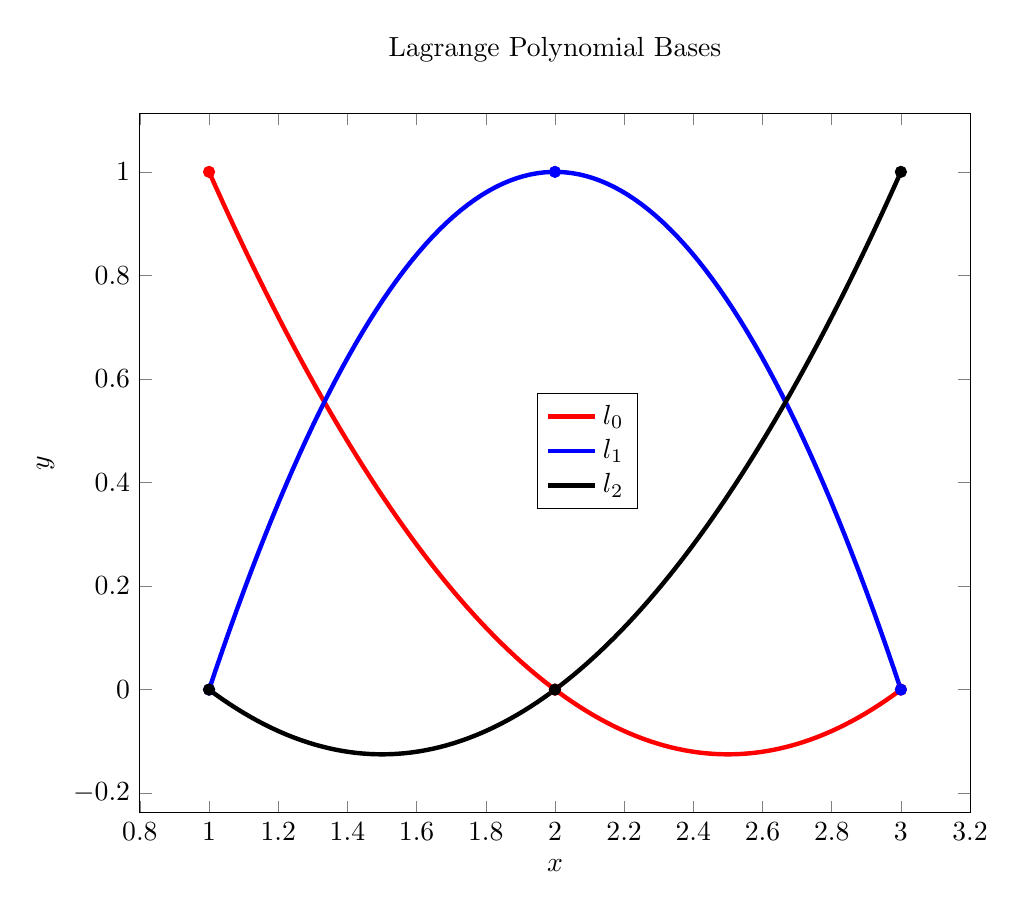
\begin{tikzpicture}
		        \begin{axis}[
		        		title style={at={(0.5,1.1)},anchor=north},
					title = Lagrange Polynomial Bases,
		            xlabel = $x$,
		            ylabel = $y$,
				  	width=\linewidth,
			  	    legend style={at={(0.6,0.6)},anchor=north east},
		            declare function={
		                l0(\x) = ( (\x - 2)*(\x - 3) ) / ( (1 - 2)*(1 - 3) );
		                l1(\x) = ( (\x - 1)*(\x - 3) ) / ( (2 - 1)*(2 - 3) );
		                l2(\x) = ( (\x - 1)*(\x - 2) ) / ( (3 - 1)*(3 - 2) );
		            }
		        ]
		            
		            % Bases Functions
		            \addplot[ultra thick, red, domain=1:3, samples=100] {l0(\x)};
					\addplot[only marks, red, samples at={1, 2, 3}]{l0(\x)};
		            
		            \addplot[ultra thick, blue, domain=1:3, samples=100] {l1(\x)};
					\addplot[only marks, blue, samples at={1, 2, 3}]{l1(\x)};
			            
		            \addplot[ultra thick, domain=1:3, samples=100] {l2(\x)};
					\addplot[only marks, samples at={1, 2, 3}]{l2(\x)};
				
					\legend{$l_0$, ,$l_1$, ,$l_2$,}
	
		        \end{axis}
		    \end{tikzpicture}
	    \end{subfigure}
	    \hfill
	    \begin{subfigure}{0.47\linewidth}
			\centering
		    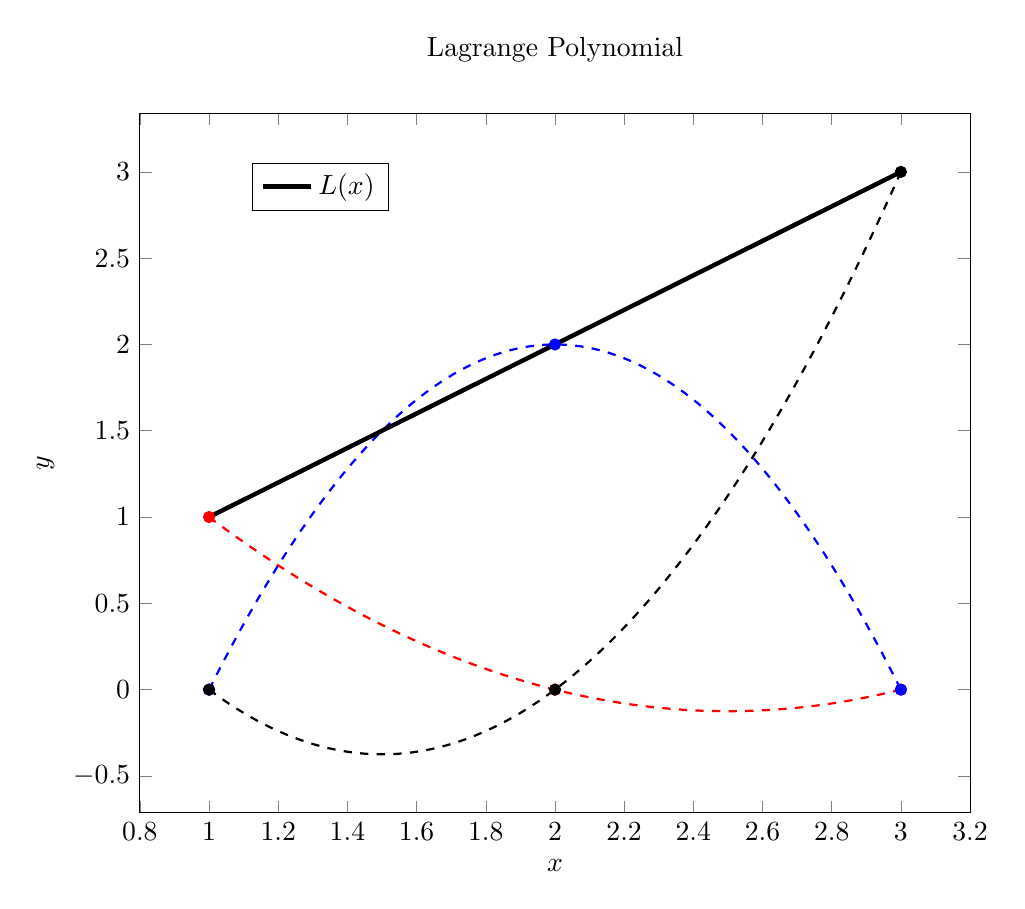
\begin{tikzpicture}
		        \begin{axis}[
		        		title style={at={(0.5,1.1)},anchor=north},
					title = Lagrange Polynomial,
		            xlabel = $x$,
		            ylabel = $y$,
				  	width=\linewidth,
			  	    legend style={at={(0.3,0.93)},anchor=north east},
		            declare function={
		                l0(\x) = ( (\x - 2)*(\x - 3) ) / ( (1 - 2)*(1 - 3) );
		                l1(\x) = ( (\x - 1)*(\x - 3) ) / ( (2 - 1)*(2 - 3) );
		                l2(\x) = ( (\x - 1)*(\x - 2) ) / ( (3 - 1)*(3 - 2) );
		            }
		        ]
		            
		            % Bases Functions
		            \addplot[thick, dashed, red, domain=1:3, samples=100] {1*l0(\x)};
					\addplot[only marks, red, samples at={1, 2, 3}]{1*l0(\x)};
		            
		            \addplot[thick, dashed, blue, domain=1:3, samples=100] {2*l1(\x)};
					\addplot[only marks, blue, samples at={1, 2, 3}]{2*l1(\x)};
	
		            
		            \addplot[thick, dashed, domain=1:3, samples=100] {3*l2(\x)};
					\addplot[only marks, samples at={1, 2, 3}]{3*l2(\x)};
					
					% Lagrange Polynomial				
		            \addplot[ultra thick, domain=1:3, samples=100] {1*l0(\x)+ 2*l1(\x) + 3*l2(\x)};
		            
					\legend{ , , , , , , $L(x)$}

		        \end{axis}
		    \end{tikzpicture}
	    \end{subfigure}
	    \caption{Lagrange Polynomial and its Bases}
	\end{adjustwidth}
	\end{figure}

\end{document}